\section{Basic Benchmarks}
\label{eval:variables}

To evaluate performance of the basic building blocks, we have designed a scenario that
selects one of a list of 100 000 members. With the \cc{oneOf} function, there is already
a constraint specifying that the cardinality of the selection is 1. From there, we
generate large numbers of additional meaningless constraints. Given that finding a valid
solution is trivial, results of this test provide information about per-constraint
processing time and memory consumption.

\medskip

To evaluate simple constraints, we generate a number of \cc{constraint} statements
specifying that selection cardinality must be smaller than $i$ for an increasing $i$. In
the constraints test case, the total number of constraints $N$ goes from 50~000 to
1~000~000.

\medskip

To evaluate \cc{Logical} expressions, we generate the following expression:
\begin{lstlisting}[style=snippet]
val condition: LogicalBoolVar = role.cardinality === 1
condition && condition && condition && /* ... repeated N times */
\end{lstlisting}
\cc{condition} creates a single \cc{BoolVar} in the solver, and the repeated use of the
\dop{&&} operator constructs an unbalanced tree of \cc{LogOp} operations of a specified
length. In this test case, $N$ goes from 500 to 10~000.

\medskip

To evaluate \cc{Integer} expressions, we generate \cc{IntVar}s by repeating idempotent
arithmetic operations. As explained in section~\ref{impl:solver:arithm}, every
arithmetic operation creates a new \cc{IntVar}. As the starting value, we use the
selection cardinality, and repeatedly add 15 to it and then subtract 15 from it $N$
times. Finally, we post a constraint that the selection cardinality must be equal to the
new value, so that the solver is forced to propagate the results of all the individual
calculations. In this test case, $N$ also goes from 500 to 10~000.

Every configuration of every test case runs 100 times.

\medskip

Figure~\ref{fig:variables:time} shows timing results. Each point represents median time
to solve a configuration of a given size. Standard deviation across runs was under
150~ms in most cases, so we choose not to display it in the graph.

\begin{figure}[t]
    \centering
    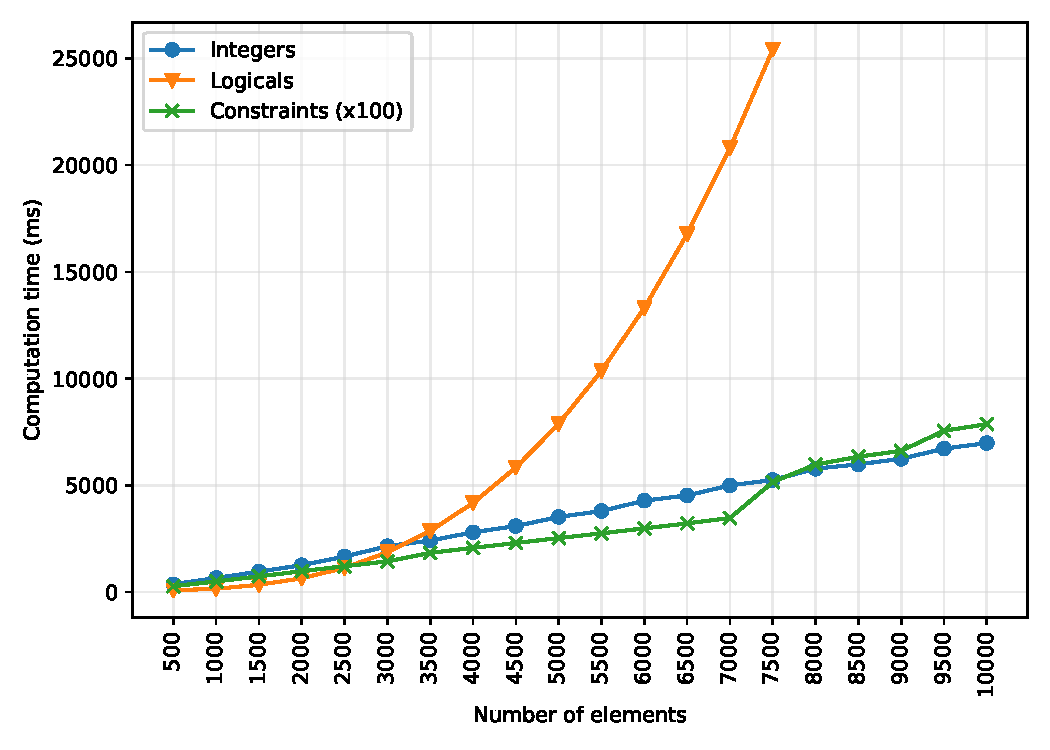
\includegraphics[width=1\linewidth]{img/variables.pdf}
    \caption{Computation times for basic building blocks}
    \label{fig:variables:time}
\end{figure}

Computation time for constraints grows linearly with the total number of constraints,
and 750~000 constraints can be processed in about 5 seconds. This would match the
intuition that the solver needs to evaluate each constraint once to ensure that the
tested solution is valid.

An interesting point is the discontinuity around the 750~000 mark. This is most likely
caused by the corresponding discontinuity in memory usage, as discussed below.

Computation time for integers also grows linearly, which matches the intuition that the
sequence of arithmetic operations must be propagated in linear time. The results also
closely follow the time measured for simple constraints. Each point represents two
arithmetic operations per element, so we can conclude that each arithmetic operation
takes roughly as much processing time as 50 simple constraints.

Computation time for logical operations grows quadratically and runs out of the allotted
30-second time limit at 8~000 operations. A \cc{Logical} operation does not create new
variables in the solver, and the full expression is posted as a single constraint. The
quadratic behavior comes from an inefficiency in Choco's CNF normalization, which does
not deal well with the unbalanced expression we are submitting. Still, 4~000 logical
operations can be done under 5 seconds.

\medskip

Figure~\ref{fig:variables:mem} shows peak memory usages. Each point represents a maximum
over the configuration runs. Memory usage data has an extremely high variance, sometimes
on the order of hundreds of megabytes, which we chalk up to the unreliability of our
measurements. Nevertheless, the maxima paint a clear picture.

\begin{figure}[t]
    \centering
    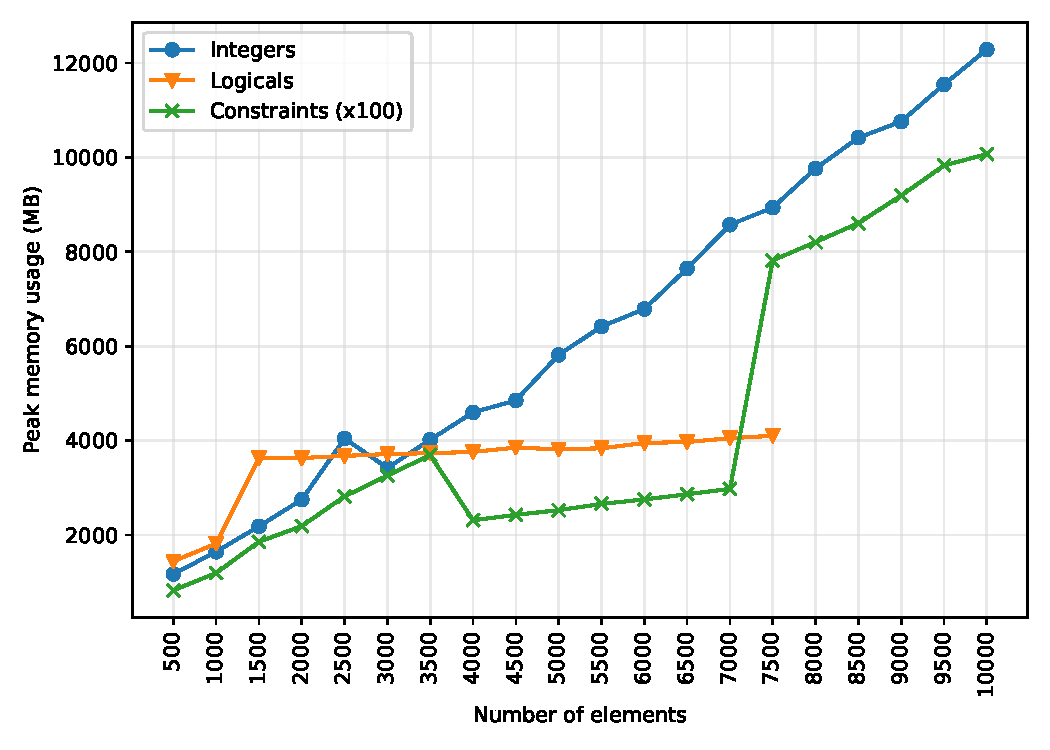
\includegraphics[width=1\linewidth]{img/variablemem.pdf}
    \caption{Memory consumption for basic building blocks}
    \label{fig:variables:mem}
\end{figure}

Memory usage for constraints grows linearly, but shows a distinct discontinuity between
400~000 and 700~000 elements. As noted above, this corresponds to a discontinuity in
processing time. We do not have an explanation for this behavior. However, the
discontinuity starts before memory usage reaches 4~GB and returns to original projection
at around 8~GB. We therefore hypothesize that this could be an artifact of JVM memory
allocator behavior, or perhaps a custom allocator in Choco.

Memory usage for integers also grows linearly, in a much more predictable manner. We
note that in this test case, the recorded peak usage resembles the actual usage more
closely than in other tests. In previous experiments, when only 4 GB were allocated to
the JVM, the integer test case ran out of memory at around 7~500 elements, and
computation time started to rise sharply around the 4~500 mark --- presumably due to
memory pressure and the need to run GC during the computation. The other test cases did
not run into similar problems; GC runs were causing timing jitter, but other than that,
the constraint test case continued linearly until 950~000 elements, and the logical
operation test case was unaffected.

The logical operation test case reaches a plateau at the 1~500 mark, rising only very
slowly in subsequent configurations. We expect that this corresponds to some
pre-allocated internal array whose size is sufficient for all our configurations; given
that the first jump is from 2 GB to 4 GB, it is possible that at some larger
configuration the pre-allocated array would grow twice as large again. The \cc{LogOp}
tree and associated data is very small in comparison.
